\pdfoutput=1
\PassOptionsToPackage{pdftex,
pdfversion=1.7,
pdfencoding=auto,
pdfnewwindow=true,
pdfusetitle=true,
%psdextra=true,
%pdftoolbar=true,
%pdfmenubar=true,
bookmarks=true,
bookmarksnumbered=true,
bookmarksopen=true,
pdfpagemode=UseThumbs,
bookmarksopenlevel=1,
pdfpagelabels=false,
breaklinks=true
}{hyperref}
\PassOptionsToPackage{usenames,dvipsnames,table}{xcolor}
\documentclass[aps,english,superscriptaddress,onecolumn,twoside,longbibliography,pra,floatfix,fleqn,nofootinbib]{revtex4-1}%

% packages
\usepackage[OT1]{fontenc}
\usepackage{amsfonts}
\usepackage{amssymb}
\usepackage{amsthm}
\usepackage[intlimits,fleqn]{amsmath}
\usepackage{bm}
\usepackage{graphicx}
%\usepackage{adjustbox}
\usepackage[normalem]{ulem} %for sout
\usepackage{paralist}
\usepackage{microtype}
\usepackage{float}% (not with floatrow)
\usepackage{wrapfig}
\usepackage{array}
\usepackage{ragged2e}%for justifying text in tables
\usepackage{tabularx}
\usepackage{booktabs}
%\usepackage{showkeys}
\usepackage[intlimits,fleqn]{mathtools} %for mathclap and prescript and more. Learning to love this package. And DeclarePairDelimeter!

% tables stuff
\newcolumntype{R}{>{\raggedleft\arraybackslash}X}
\newcolumntype{C}{>{\centering\arraybackslash}X}
\newcolumntype{L}{>{\raggedright\arraybackslash}X}
\newcolumntype{J}{>{\justifying\arraybackslash}X}
\usepackage{adjustbox}
\usepackage{multirow}
\newcolumntype{T}[2]{%
    >{\adjustbox{angle=#1,lap=\width-(#2)}\bgroup}%
    l%
    <{\egroup}%
}
\setcounter{MaxMatrixCols}{30}

\usepackage{verbatim} %for comment command

% colours and hyperlink stuff
\usepackage[usenames,dvipsnames,table]{xcolor}
\definecolor{purple}{RGB}{128,0,128}
\definecolor{ultramarine}{RGB}{63, 0, 255}
\definecolor{medblue}{RGB}{0, 0, 100}
\definecolor{panblue}{RGB}{0,24,150}
\definecolor{carmine}{RGB}{150, 0, 24}
\definecolor{gray}{RGB}{150, 150, 150}
\usepackage[pdftex,pdfversion=1.7,pdfencoding=auto,pdfnewwindow=true,pdfusetitle=true,bookmarks=true,bookmarksnumbered=true,bookmarksopen=true,pdfpagemode=UseThumbs,bookmarksopenlevel=1,pdfpagelabels=false,breaklinks=true]{hyperref}
\hypersetup{colorlinks,
linkcolor=carmine,
citecolor=medblue,
urlcolor=panblue,
anchorcolor=OliveGreen}



% coloured text
\newcommand*{\mred}[1]{{\color{RawSienna}{\mathbf{#1}}}}
\newcommand*{\mgreen}[1]{{\color{OliveGreen}{\mathbf{#1}}}}
\newcommand*{\tred}[1]{{\color{carmine}{\textbf{#1}}}}
\newcommand*{\tblue}[1]{{\color{MidnightBlue}{\textbf{#1}}}}
\newcommand*{\tpurp}[1]{{\color{Plum}{{#1}}}}

% cleveref stuff
\usepackage[capitalise]{cleveref}
\Crefname{eqs}{Eqs.}{Eqs.}
\creflabelformat{eqs}{(#2#1#3)}
\crefrangelabelformat{equation}{(#3#1#4-#5#2#6)}
\Crefmultiformat{equation}{Eqs.~(#2#1#3}{,#2#1#3)}{,#2#1#3}{,#2#1#3)}
\crefrangelabelformat{eqs}{(#3#1#4-#5#2#6)}
\Crefmultiformat{eqs}{Eqs.~(#2#1#3}{,#2#1#3)}{,#2#1#3}{,#2#1#3)}
\Crefname{example}{Example}{Examples}
\Crefname{section}{Sec.}{Secs.}



% theorem environments
\newtheorem{theorem}{Theorem}
\newtheorem{lemma}[theorem]{Lemma}
\newtheorem{claim}[theorem]{Claim}
\newtheorem{conjecture}[theorem]{Conjecture}
\newtheorem{corollary}[theorem]{Corollary}
\newtheorem{definition}[theorem]{Definition}
\theoremstyle{definition}
%\newtheorem{example}{Example}
\newtheorem{exercise}{Exercise}
\newtheorem{notation}[theorem]{Notation}
\newtheorem{problem}[theorem]{Problem}
\newtheorem{remark}[theorem]{Remark}

\newcounter{example}[section]
\newenvironment{example}[1][]{\refstepcounter{example}\par\medskip
   \noindent \textbf{Example~\theexample}\hspace{1em}\rmfamily#1}{\par\medskip\par}
\Crefname{example}{Example}{Examples}
\creflabelformat{example}{#2#1#3}
\crefrangelabelformat{example}{#3#1#4-#5#2#6}
\Crefmultiformat{example}{Examples~#2#1#3}{, #2#1#3}{, #2#1#3 }{and #2#1#3}
\renewcommand{\theexample}{\arabic{example}}

% macros for our notation
\newcommand{\p}[2][]{{P_{#1}}\parenths{#2}}
\newcommand{\pfunc}[1]{P_{#1}}
\newcommand{\An}[2][]{{\mathsf{An}_{#1}}\parenths{#2}}
\newcommand{\Pa}[2][]{{\mathsf{Pa}_{#1}}\parenths{#2}}
\newcommand{\Ch}[2][]{{\mathsf{Ch}_{#1}}\parenths{#2}}
\newcommand{\SmallNamedFunction}[3][]{\operatorname{\mathsf{#2}}_{#1}\parenths{#3}}
\newcommand{\subgraph}[2][]{\SmallNamedFunction[#1]{SubDAG}{#2}}
\newcommand{\ansubgraph}[2][]{\SmallNamedFunction[#1]{AnSubDAG}{#2}}
\newcommand{\nodes}[1]{\SmallNamedFunction{Nodes}{#1}}
\newcommand{\obsnodes}[1]{\SmallNamedFunction{ObservedNodes}{#1}}
\newcommand{\latnodes}[1]{\SmallNamedFunction{LatentNodes}{#1}}
\newcommand{\inflations}[1]{\SmallNamedFunction{Inflations}{#1}}
\newcommand{\DAG}[1]{\SmallNamedFunction{DAG}{#1}}
\newcommand{\edges}[1]{\SmallNamedFunction{Edges}{#1}}
\newcommand{\aindep}{\perp} % for d-separation
\newcommand{\indep}{\perp\!\!\!\!\perp} % (conditional) independence
\newcommand{\cramp}[1]{\ensuremath{\mathord{#1}}}
\newcommand{\eql}{\cramp{=}}
\DeclarePairedDelimiter{\parens}{\lparen}{\rparen}
\DeclarePairedDelimiter{\parenths}{\lparen}{\rparen}
\DeclarePairedDelimiter{\braces}{\lbrace}{\rbrace}
\DeclarePairedDelimiter{\bracks}{\lbrack}{\rbrack}
\DeclarePairedDelimiter{\expec}{\langle}{\rangle}
\newcommand{\brackets}[1]{\braces*{#1}}

% more vertical spacing in multiline equations
\setlength{\jot}{6pt}





\begin{document}

\title{Expressible sets and expressible assignments}

\author{RWS}

%\date{}                                           % Activate to display a given date or no date

\maketitle
%\section{}
%\subsection{}

\section{Expressible sets}

\begin{example}[\tred{Incompatibility of Pienaar distribution with DAG \#16}]
\label{example:Pienaar}

Consider the DAG of \cref{fig:GDAG16}.  Henson, Lal and Pusey showed that this DAG is a candidate for being `interesting', that is, the compatible distributions satisfy constraints over and above the conditional independence relations that follow from d-separation relations in the DAG. 

% i.e. for which the set of distributions that are compatible with it is a strict subset of those with conditional independence relations that are implied by the d-separation criterion. 

% Pienaar subsequently showed that this was the case by demostrating that the following distribution is incompatible with the DAG:

\begin{figure}[htb]
\centering
\begin{minipage}[t]{0.4\linewidth}
\centering
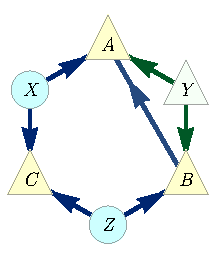
\includegraphics[scale=1]{scen16DAG.pdf}
\caption{DAG \#16 in Ref.~\cite{pusey2014gdag}.}\label{fig:GDAG16}
\end{minipage}
\hfill
\begin{minipage}[t]{0.5\linewidth}
\centering
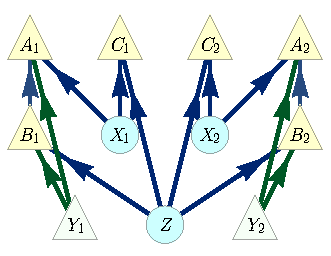
\includegraphics[scale=1]{scen16InflationDAG.pdf}
\caption{The Rocket inflation of \cref{fig:GDAG15}.}\label{fig:Inflated15}
\end{minipage}
\end{figure}

\citet{pianaar2016interesting} identified a distribution which satisfies the CI relations among the observed variables in DAG \#16, namely, $Y\indep C$ and $A\indep B | Y$~\cite{pusey2014gdag}, but is nonetheless incompatible with it:
\begin{align}\label{eq:pienaardistro}
    P^{\text{Pien}}_{A B C Y}:=\frac{[0000]+[0110]+[0001]+[1011]}{4},\quad\text{i.e.,}\quad P^{\text{Pien}}_{Y\! A B C}(y a b c):=\begin{cases}\tfrac{1}{4}&\text{if }  y\cdot c = a \text{ and }  (y \oplus 1)\cdot c = b, \\ 0&\text{otherwise}.\end{cases}
\end{align}
In words, if $Y=0$, then $B$ and $C$ are in a maximally correlated state, while $A$ takes the value 0, while if $Y=1$, then $A$ and $C$ are maximally correlated, while $B$ takes the value $0$.

Here, we will establish this incompatibility using the inflation technique.  To do so, we use the Parachute inflation of the Modified Triangle scrnario, depicted in \cref{fig:Inflated15}.  
The injectable sets include $\brackets{A_1 B_1 C_1 Y_1}$ and $\brackets{A_2 B_1 C_2 Y_1}$.  They share the same  image on the original DAG, namely, the set of all observed variables, $\brackets{ABCY}$. It follows that
\begin{align}
P_{A_1 B_1 C_1 Y_1} = P_{A_2 B_1 C_2 Y_1} =P^{\text{Pien}}_{ABCY}.
\end{align}

If $P^{\text{Pien}}_{ABCY}$ is compatible with the Modified Triangle Scenario, then by Lemma ?, $P_{A_1 B_1 C_1 Y_1}$ and $ P_{A_2 B_1 C_2 Y_1}$ are compatible with the Parachute inflation of the Modified Triangle Scenario.  To show that $P^{\text{Pien}}_{ABCY}$ is {\em incompatible} with the Modified Triangle Scenario, we assume do so, we assume that $P_{A_1 B_1 C_1 Y_1}$ and $ P_{A_2 B_1 C_2 Y_1}$ are compatible with the Parachute inflation of the Modified Triangle Scenario and derive a contradiction.

%With a slight rewriting of Eq.~\ref{eq:pienaardistro}, we have
Note first that we can rewrite Eq.~\ref{eq:pienaardistro} as
\begin{align}
P_{A B C Y}= \frac{1}{2}([00]_{BC}+[11]_{BC})[0]_A [0]_Y + \frac{1}{2}([00]_{AC}+[11]_{AC}) [0]_B [1]_Y
\end{align}
It follows that
\begin{align}
P_{A_1 C_1 | Y_1=1} = \frac{1}{2}([00]_{A_1 C_1}+[11]_{A_1 C_1}),\label{A1C1Y1e1}\\
P_{A_2 C_2 |Y_1=1} = \frac{1}{2}([00]_{A_2 C_2}+[11]_{A_2 C_2}).\label{A2C2Y1e1}
\end{align}
and that 
\begin{align}
P_{B_1 C_1 | Y_1=0} = \frac{1}{2}([00]_{B_1 C_1}+[11]_{B_1 C_1}),\label{B1C1Y1e0}\\
P_{B_1 C_2 |Y_1=0} = \frac{1}{2}([00]_{B_1 C_2}+[11]_{B_1 C_2}).\label{B1C2Y1e0}
\end{align}

Any distribution $P_{B_1 C_1 C_2 Y_1}$ which has marginals $P_{B_1 C_1 Y_1}$ and $P_{B_1 C_2 Y_1}$ that reproduce the conditional distributions of \cref{B1C1Y1e0} and \cref{B1C2Y1e0} respectively, must be such that 
\begin{align}
P_{B_1 C_1 C_2 | Y_1=0} = \frac{1}{2}([000]_{B_1 C_1 C_2}+[111]_{B_1 C_1 C_2})\label{B1C1C2Y1e0}.
\end{align}
The reason is that if $B_1$ and $C_1$ are perfectly correlated, as in \cref{B1C1Y1e0}, and $B_1$ and $C_2$ are perfectly correlated, as in \cref{B1C2Y1e0}, then $C_1$ and $C_2$ must be perfectly correlated as well.  Indeed, marginalizing \cref{B1C1C2Y1e0} over $B_1$, we obtain
\begin{align}
P_{C_1 C_2 | Y_1=0} = \frac{1}{2}([00]_{ C_1 C_2}+[11]_{C_1 C_2}).\label{C1C2Y1e0}
\end{align}

But the Parachute inflation of the Modified Triangle Scenario is such that $C_1 C_2$ and $Y_1$ are ancestrally independent, so that 
\begin{align}
P_{C_1 C_2 | Y_1} =P_{C_1 C_2},
\end{align}
and therefore $P_{C_1 C_2 | Y_1=0}=P_{C_1 C_2 | Y_1=1}$, so that we can infer from \cref{C1C2Y1e0} that
\begin{align}
P_{C_1 C_2 | Y_1=1} = \frac{1}{2}([00]_{ C_1 C_2}+[11]_{C_1 C_2})\label{C1C2Y1e1}.
\end{align}

Finally, we note that any distribution $P_{A_1 A_2 C_1 C_2 Y_1}$ which has marginals $P_{A_1 C_1 Y_1}$, $P_{A_2 C_2 Y_1}$, and $P_{C_1 C_2 Y_1}$ that reproduce the conditional distributions of \cref{A1C1Y1e1}, \cref{A2C2Y1e1} and \cref{C1C2Y1e1} respectively must be such that 
\begin{align}
P_{A_1 A_2 C_1 C_2 | Y_1=1} = \frac{1}{2}([0000]_{A_1 A_2 C_1 C_2}+[1111]_{A_1 A_2 C_1 C_2})\label{A1A2C1C2Y1e1}.
\end{align}
The reason is that if $A_1$ and $C_1$ are perfectly correlated, as in \cref{A1C1Y1e1}, and $A_2$ and $C_2$ are perfectly correlated, as in \cref{A2C2Y1e1}, and $C_1$ and $C_2$ are perfectly correlated, as in \cref{C1C2Y1e1}, then $A_1$ and $A_2$ must be perfectly correlated as well. 

Marginalizing \cref{A1A2C1C2Y1e1} over $C_1 C_2$, we obtain
\begin{align}
P_{A_1 A_2  | Y_1=1} = \frac{1}{2}([00]_{A_1 A_2}+[11]_{A_1 A_2})\label{A1A2Y1e1}.
\end{align}

Finally, we note that in the Parachute inflation of the Modified Triangle Scenario, $A_1$ is d-separated from $A_2$ given $Y_1$, which implies that $P_{A_1 A_2  | Y_1}=P_{A_1 | Y_1}P_{A_2  | Y_1}$.  This is inconsistent with \cref{A1A2Y1e1}, so we have derived a contradiction.

\end{example}
\color{black}



\end{document}  